\begin{center}

\includegraphics[width=0.3\textwidth]{content/3/chapter6/images/7.png}\\
Cippi在研究原子
\end{center}

C++20中,原子操作和类型得到了一些重要的扩展,最重要的可能就是原子引用和原子智能指针。

\subsubsubsection{6.2.1\hspace{0.2cm}std::atomic\_ref}

类模板std::atomic\_ref可对引用的对象进行原子操作。

原子对象的并发写入和读取可避免数据竞争。引用对象的生命周期必须超过atomic\_ref的生命周期。当atomic\_ref正在访问一个对象时,对该对象的所有其他访问必须使用atomic\_ref。此外,atomic\_ref访问对象的子对象不能被另一个atomic\_ref访问。

\hspace*{\fill} \\ %插入空行
\noindent
\textbf{6.2.1.1\hspace{0.2cm}动机}

等一下!您可能认为在原子中使用引用就可以完成这项工作,但事实并不是这样。

下面的程序中,实现了一个ExpensiveToCopy类,它包括一个计数器。计数器并发递增几个线程,所以counter必须得到保护。

\hspace*{\fill} \\ %插入空行
\noindent
\textbf{使用原子引用}
\begin{lstlisting}[style=styleCXX]
// atomicReference.cpp

#include <atomic>
#include <iostream>
#include <random>
#include <thread>
#include <vector>

struct ExpensiveToCopy {
	int counter{};
};

int getRandom(int begin, int end) {
	
	std::random_device seed; // initial seed
	std::mt19937 engine(seed()); // generator
	std::uniform_int_distribution<> uniformDist(begin, end);
	
	return uniformDist(engine);
}

void count(ExpensiveToCopy& exp) {

	std::vector<std::thread> v;
	std::atomic<int> counter{exp.counter};
	
	for (int n = 0; n < 10; ++n) {
		v.emplace_back([&counter] {
			auto randomNumber = getRandom(100, 200);
			for (int i = 0; i < randomNumber; ++i) { ++counter; }
		});
	}
	
	for (auto& t : v) t.join();

}

int main() {
	
	std::cout << '\n';
	
	ExpensiveToCopy exp;
	count(exp);
	std::cout << "exp.counter: " << exp.counter << '\n';
	
	std::cout << '\n';

}
\end{lstlisting}

变量exp(第42行)是复制成本较高的对象。出于对性能的考虑,count(第22行)通过引用获取exp。函数count使用exp.counter初始化std::atomic<int>(第25行)。下面的代码行创建了10个线程(第27行),每个线程执行Lambda表达式,该表达式通过引用接受counter。Lambda表达式获得100到200之间的随机数(第29行),并以相同的频率递增计数器。函数getRandom(第13行)从初始种子开始,并通过随机数生成器\href{https://en.wikipedia.org/wiki/Mersenne_Twister}{马特赛特旋转演算法}创建一个在100到200之间的均匀分布数。

最后,exp.counter(第44行)的近似值应该是1500,因为10个线程平均增加150倍。\href{https://wandbox.org/}{Wandbox在线编译器}上执行程序会给我一个令人惊讶的结果。

\begin{center}
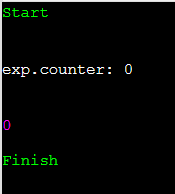
\includegraphics[width=0.2\textwidth]{content/3/chapter6/images/8.png}\\
\end{center}

计数器为0。发生了什么?问题在第25行。表达式std::atomic counter\{exp. counter\}创建一个副本。下面的小程序说明了这个问题。

\hspace*{\fill} \\ %插入空行
\noindent
\textbf{复制引用}
\begin{lstlisting}[style=styleCXX]
// atomicRefCopy.cpp

#include <atomic>
#include <iostream>

int main() {

	std::cout << '\n';
	
	int val{5};
	int& ref = val;
	std::atomic<int> atomicRef(ref);
	++atomicRef;
	std::cout << "ref: " << ref << '\n';
	std::cout << "atomicRef.load(): " << atomicRef.load() << '\n';
	
	std::cout << '\n';

}
\end{lstlisting}

第13行中的增量操作没有处理引用引用(第11行),ref的值没有改变。

\begin{center}
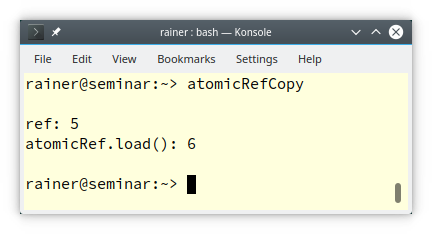
\includegraphics[width=0.5\textwidth]{content/3/chapter6/images/9.png}\\
\end{center}

将std::atomic<int>替换为std::atomic\_ref<int>可以解决这个问题。

\begin{lstlisting}[style=styleCXX]
// atomicRef.cpp

#include <atomic>
#include <iostream>
#include <random>
#include <thread>
#include <vector>

struct ExpensiveToCopy {
	int counter{};
};

int getRandom(int begin, int end) {
	std::random_device seed; // initial randomness
	std::mt19937 engine(seed()); // generator
	std::uniform_int_distribution<> uniformDist(begin, end);
	
	return uniformDist(engine);
}

void count(ExpensiveToCopy& exp) {
	
	std::vector<std::thread> v;
	std::atomic_ref<int> counter{exp.counter};
	
	for (int n = 0; n < 10; ++n) {
		v.emplace_back([&counter] {
			auto randomNumber = getRandom(100, 200);
			for (int i = 0; i < randomNumber; ++i) { ++counter; }
		});
	}

	for (auto& t : v) t.join();
}

int main() {
	
	std::cout << '\n';
	
	ExpensiveToCopy exp;
	count(exp);
	std::cout << "exp.counter: " << exp.counter << '\n';
	
	std::cout << '\n';
}
\end{lstlisting}

现在,counter的值和预期的一样:

\begin{center}
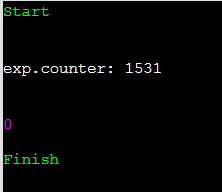
\includegraphics[width=0.2\textwidth]{content/3/chapter6/images/10.png}\\
\end{center}

为了与\href{https://en.cppreference.com/w/cpp/atomic/atomic}{std::atomic}保持一致,类型std::atomic\_ref也可以特化,并支持内置数据类型的特化。

\hspace*{\fill} \\ %插入空行
\noindent
\textbf{6.2.1.2\hspace{0.2cm}std::atomic\_ref的特化}

可以将std::atomic\_refte特化为自定义的类型,对指针类型使用偏特化,对算术类型(如整型或浮点型)使用全特化。

\hspace*{\fill} \\ %插入空行
\noindent
\textbf{6.2.1.2.1\hspace{0.2cm}主模板}

主模板std::atomic\_ref可以用\href{https://en.cppreference.com/w/cpp/types/is_trivially_copyable}{TriviallyCopyable}类型T进行实例化。

\begin{lstlisting}[style=styleCXX]
struct Counters {
	int a;
	int b;
};

Counter counter;
std::atomic_ref<Counters> cnt(counter);
\end{lstlisting}

\hspace*{\fill} \\ %插入空行
\noindent
\textbf{6.2.1.2.2\hspace{0.2cm}指针类型的偏特化}

标准为指针类型提供了偏特化:std::atomic\_ref<T*>。

\hspace*{\fill} \\ %插入空行
\noindent
\textbf{6.2.1.2.3\hspace{0.2cm}算术类型的特化}

该标准为整型和浮点型提供了特化:

\begin{itemize}
\item 
字符类型:char、char8\_t(C++20)、char16\_t、char32\_t和wchar\_t

\item 
标准有符号整型类型:有符号char、short、int、long和long long

\item 
标准的无符号整型类型:unsigned char、unsigned short、unsigned int、unsigned long和unsigned long

\item 
头文件\href{http://en.cppreference.com/w/cpp/header/cstdint}{<cstdint>}中定义的其他整数类型:
\begin{itemize}
\item 
int8\_t, int16\_t, int32\_t和int64\_t (8,16,32和64位有符号整数)

\item 
uint8\_t, uint16\_t, uint32\_t和uint64\_t (8,16,32和64位无符号整数)

\item 
int\_fast8\_t, int\_fast16\_t, int\_fast32\_t和int\_fast64\_t (8,16,32和64位的快速有符号整数)

\item 
uint\_fast8\_t, uint\_fast16\_t, uint\_fast32\_t和uint\_fast64\_t(8,16,32和64位快速无符号整数)

\item 
int\_least8\_t, int\_least16\_t, int\_least32\_t和int\_least64\_t (8,16,32和64位的最小有符号整数)

\item 
uint\_least8\_t, uint\_least16\_t, uint\_least32\_t和uint\_least64\_t (8,16,32和64位的最小无符号整数)

\item 
intmax \_t和uintmax\_t (最大有符号整数和无符号整数)

\item 
intptr\_t和uintptr\_t (有符号和无符号整数,用于保存指针)
\end{itemize}

\item 
标准浮点类型:浮点型、双精度浮点型和长双精度浮点型
\end{itemize}

\hspace*{\fill} \\ %插入空行
\noindent
\textbf{6.2.1.2.4\hspace{0.2cm}原子操作}

下面是atomic\_ref的操作列表。

\begin{table}[H]
\centering
\begin{tabular}{ll}
\textbf{函数} & \textbf{描述}                                                             \\ \hline
is\_lock\_free    & 检查atomic\_ref对象是否无锁。                                   \\
load              & 原子地返回引用对象的值。                           \\ \hline
store             & 原子地用非原子值替换引用对象的值。        \\ \hline
exchange          & 原子地用新值替换引用对象的值。       \\ \hline
\begin{tabular}[c]{@{}l@{}}compare\_exchange\_strong\\ compare\_exchange\_weak\end{tabular} &
原子地比较并最终交换引用对象的值。 \\ \hline
\begin{tabular}[c]{@{}l@{}}fetch\_add, += \\ fetch\_sub, -=\end{tabular} &
原子地对引用的对象进行加(减)法。 \\ \hline
\begin{tabular}[c]{@{}l@{}}fetch\_or, |= \\ fetch\_and, \&= \\ fetch\_xor, \textasciicircum{}=\end{tabular} &
对引用的对象原子地执行按位(AND、OR和XOR)操作。 \\ \hline
++, --            & 递增或递减(递增前或递增后)引用对象。 \\ \hline
\begin{tabular}[c]{@{}l@{}}notify\_one \\ notify\_all\end{tabular} &
\begin{tabular}[c]{@{}l@{}}解除阻塞所有原子等待操作。\\ 解除单个原子等待操作。\end{tabular} \\ \hline
wait &
\begin{tabular}[c]{@{}l@{}}阻塞直到得到通知。 \\将自身与旧值进行比较,以防止为唤醒和未唤醒。 \\ 若该值与旧值不同,则直接返回。\end{tabular} \\ \hline
\end{tabular}
\end{table}


复合赋值运算符(+=,-=,|=,\&=,或\^{}=)返回新值,fetch方式返回旧值。

每个函数都支持一个内存序参数,其默认值是std::memory\_order\_seq\_cst,也可以使用std::memory\_order\_relax,std::memory\_order\_consume,std::memory\_order\_acquire,std::memory\_order\_release或std::memory\_order\_acq\_rel。compare\_exchange\_strong和compare\_exchange\_weak方法有两个内存序参数,一个用于成功情况,另一个用于失败情况。两个调用若相等则执行原子交换,不相等则执行原子加载。在成功的情况下,返回true,否则返回false。若只显式地提供一种内存序,则成功和失败的情况都使用这个内存序。下面是\href{https://en.cppreference.com/w/cpp/atomic/memory_order}{内存序}的详细信息。

当然,并不是所有操作都适用于std::atomic\_ref引用的所有类型。该表显示了所有原子操作的列表,具体取决于std::atomic\_ref引用的类型。

\begin{center}
所有原子操作,取决于std::atomic\_ref引用的类型
\end{center}

\begin{table}[H]
\centering
\begin{tabular}{lllll}
\textbf{函数} &
\textbf{atomic\_ref\textless{}T\textgreater{}} &
\textbf{atomic\_ref\textless{}integral\textgreater{}} &
\textbf{atomic\_ref\textless{}floating\textgreater{}} &
\textbf{atomic\_ref\textless{}T*\textgreater{}} \\ \hline
is\_lock\_free                  & yes & yes & yes & yes \\
load                            & yes & yes & yes & yes \\
store                           & yes & yes & yes & yes \\
exchange                        & yes & yes & yes & yes \\
compare\_exchange\_strong       & yes & yes & yes & yes \\
compare\_exchange\_weak         & yes & yes & yes & yes \\
fetch\_add, +=                  &     & yes & yes & yes \\
fetch\_sub, -=                  &     & yes & yes & yes \\
fetch\_or, |=                   &     & yes &     &     \\
fetch\_and, \&=                 &     & yes &     &     \\
fetch\_xor, \textasciicircum{}= &     & yes &     &     \\
++, --                          &     & yes &     & yes \\
notify\_one                     & yes & yes & yes & yes \\
notify\_all                     & yes & yes & yes & yes \\
wait                            & yes & yes & yes & yes
\end{tabular}
\end{table}

\subsubsubsection{6.2.2\hspace{0.2cm}原子智能指针}

\href{https://en.cppreference.com/w/cpp/memory/shared_ptr}{std::shared\_ptr}是由一个控制块及其资源组成。控制块是线程安全的,但对资源的访问不是。所以修改引用计数器是一个原子操作,从而可以保证资源只删除一次。

\begin{tcolorbox}[breakable,enhanced jigsaw,colback=blue!5!white,colframe=blue!75!black,title={线程安全的重要性}]
	
先来强调一下,std::shared\_ptr具有定义良好的多线程语义非常重要。乍一看,对于多线程代码来说,使用std::shared\_ptr似乎不是一个明智的选择。根据定义,它是共享和可变的,是非同步读写操作的理想候选对象,所以是未定义行为的理想候选对象。另一方面,现代C++中有一条准则:不要使用原始指针。因此,开发者应该在多线程程序中使用智能指针。
	
\end{tcolorbox}

提案\href{http://wg21.link/n4162}{N4162}直接解决了当前所面临的问题。这些问题可以归结为三点:一致性、正确性和性能。

\begin{itemize}
\item 
\textbf{一致性}:std::shared\_ptr的原子操作是非原子数据类型的唯一原子操作。

\item 
\textbf{正确性}:全局原子操作的使用很容易出错,正确的使用方式是基于规则的。很容易忘记使用原子操作——例如:使用ptr = localPtr,而不是std::atomic\_store(\&ptr, localPtr)。由于数据竞争,从而导致未定义的行为。若使用原子智能指针,类型系统将不允许这样做。

\item 
\textbf{性能}:原子智能指针与自atomic\_*函数相比有很大的优势。原子版本是为特殊用例设计的,可以在内部有一个std::atomic\_flag作为一种廉价的\href{https://en.wikipedia.org/wiki/Spinlock}{自旋锁}。没必要将指针函数的非原子版本设计为线程安全的,在单线程场景中使用原子操作没必要,并且还会有性能惩罚。
\end{itemize}

正确性可能是最重要的一个。为什么?答案就在提案中。该建议提供了线程安全的单链表,支持元素的插入、删除和搜索。并且,这个单链表以无锁的方式实现。

\hspace*{\fill} \\ %插入空行
\noindent
\textbf{6.2.2.1\hspace{0.2cm}线程安全的单链表}

\begin{center}
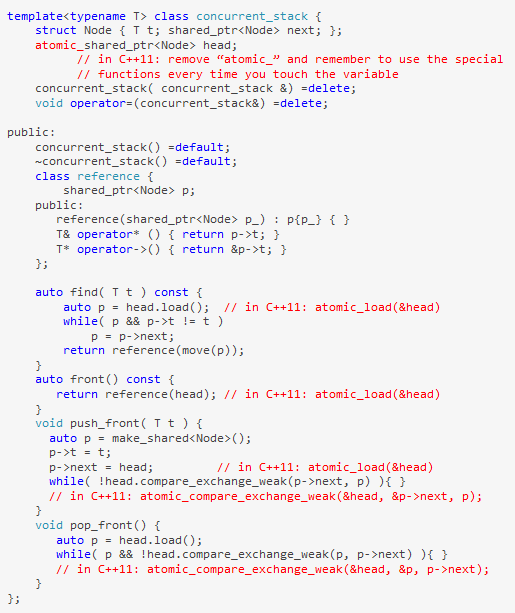
\includegraphics[width=0.8\textwidth]{content/3/chapter6/images/11.png} \\
\end{center}

C++11编译器编译程序所需的所有更改,都用红色标记。使用原子智能指针的实现要容易得多,并且不容易出错。C++20的类型系统,不允许在原子智能指针上使用非原子操作。

提案\href{http://wg21.link/n4162}{N4162}提出了新的类型std::atomic\_shared\_ptr和std::atomic\_weak\_ptr。将它们合并到ISO C++标准中,表示它们成为std::atomic的模板偏特化,即std::atomic<std::shared\_ptr<T>{}>和std::atomic<std::weak\_ptr<T>{}>。

因此,std::shared\_ptr的原子操作在C++20中弃用了。

\subsubsubsection{6.2.3\hspace{0.2cm}std::atomic\_flag扩展}

介绍C++20中的std::atomic\_flag扩展前,我想简单地提一下C++11中的std::atomic\_flag。若想了解更多细节,请阅读我关于C++11中\href{https://www.modernescpp.com/index.php/the-atomic-flag}{std::atomic\_flag}的文章。

\hspace*{\fill} \\ %插入空行
\noindent
\textbf{6.2.3.1\hspace{0.2cm}C++11}

std::atomic\_flag是一种原子布尔值,具有清态和定态的功能。简单起见,我称clear状态为false,set状态为true。clear成员函数可以将其值设置为false。使用test\_and\_set方法,可以将值设置为true并返回之前的值。ATOMIC\_FLAG\_INIT允许将std::atomic\_flag初始化为false。

std::atomic\_flag有两个重要的属性

\begin{itemize}
\item 
唯一的无锁原子类型。

\item 
更高的线程构建块抽象。
\end{itemize}

C++11中,没有成员函数要求std::atomic\_flag的当前值而不更改它,而这在C++20中有所改变。

\hspace*{\fill} \\ %插入空行
\noindent
\textbf{6.2.3.2\hspace{0.2cm}C++20的扩展}

下表展示了在C++20中std::atomic\_flag具有更强大的接口。

\begin{table}[H]
\centering
\begin{tabular}{ll}
\textbf{操作}             & \textbf{描述}                                           \\ \hline
atomicFlag.clear()          & 清除原子flag。                                        \\
\begin{tabular}[c]{@{}l@{}}atomicFlag.test\_and\_set() \\ atomicFlag.test() (C++20)\end{tabular} &
\begin{tabular}[c]{@{}l@{}}设置原子flag,并返回旧值。 \\ 返回flag的值。\end{tabular} \\
\begin{tabular}[c]{@{}l@{}}atomicFlag.notify\_one() (C++20) \\ atomicFlag.notify\_all (C++20)\end{tabular} &
\begin{tabular}[c]{@{}l@{}}通知一个等待原子flag的线程。\\ 通知所有等待原子flag的线程。\end{tabular} \\
atomicFlag.wait(bo) (C++20) & 阻塞线程,直到得到通知,将原子值改变为止。
\end{tabular}
\end{table}

调用atomicFlag.test()返回atomicFlag值而不更改它,使用std::atomic\_flag进行线程同步:atomicFlag.wait()、atomicFlag.notify\_one()和atomicFlag.notify\_all()。成员函数notify\_one或notify\_all通知一个或所有处于等待的原子flag,atomicFlag.wait(bo)需要一个布尔值bo,使用atomicFlag.wait(bo)将其阻塞,直到下一次通知或伪唤醒。然后,会检查atomicFlag的值是否等于bo,若不等于则解除阻塞。值bo用作防止伪唤醒的谓词,而伪唤醒是一种错误的通知。

与C++11相比,std::atomic\_flag的默认构造初始化为false。

根据C++标准,更强大的原子功能,可以通过互斥量来提供。因此这些原子有一个成员函数is\_lock\_free,可以用来检查原子内部是否使用了互斥量。在主流的平台上,我总是得到false的回答,但各位需要了解这一点。


\hspace*{\fill} \\ %插入空行
\noindent
\textbf{6.2.3.3\hspace{0.2cm}线程的一次性同步}

发送-接收工作流对于线程来说非常常见。这样的工作流中,接收者在Future继续工作之前等待发送者的通知。有多种方法可以实现这些工作流。C++11可以使用条件变量或promise/future对,C++20可以使用std::atomic\_flag。每种方法都有其利弊,所以我想对它们进行比较。我假设读者们并不了解条件变量,promise和future的细节。因此,这里会提供一些简短的复习内容。

\hspace*{\fill} \\ %插入空行
\noindent
\textbf{6.2.3.3.1\hspace{0.2cm}条件变量}

条件变量可以扮演发送者或接收者的角色。作为发送方,可以通知一个或多个接收方。

\begin{lstlisting}[style=styleCXX]
// threadSynchronizationConditionVariable.cpp

#include <iostream>
#include <condition_variable>
#include <mutex>
#include <thread>
#include <vector>

std::mutex mut;
std::condition_variable condVar;

std::vector<int> myVec{};

void prepareWork() {

	{
	std::lock_guard<std::mutex> lck(mut);
	myVec.insert(myVec.end(), {0, 1, 0, 3});
	}
	std::cout << "Sender: Data prepared." << '\n';
	condVar.notify_one();
}

void completeWork() {

	std::cout << "Waiter: Waiting for data." << '\n';
	std::unique_lock<std::mutex> lck(mut);
	condVar.wait(lck, []{ return not myVec.empty(); });
	myVec[2] = 2;
	std::cout << "Waiter: Complete the work." << '\n';
	for (auto i: myVec) std::cout << i << " ";
	std::cout << '\n';

}

int main() {

	std::cout << '\n';
	
	std::thread t1(prepareWork);
	std::thread t2(completeWork);
	
	t1.join();
	t2.join();
	
	std::cout << '\n';

}
\end{lstlisting}

程序有两个子线程:t1和t2,在第40行和第41行中获得负载prepareWork和completeWork。函数prepareWork(第14行)通知它已经完成了工作的准备:condVar.notify\_one()。当持有锁时,线程t2正在等待它的通知:condVar.wait(lck,[]\{return not myVec.empty();\})。等待线程总是执行相同的步骤。唤醒时,在持有锁的同时检查谓词([]\{return not myVec.empty();)。若谓词不成立,重新回到休眠状态;否则,将继续其工作。在具体的工作流中,发送线程将初始值放入std::vector(第18行),接收线程完成(第29行)。

\begin{center}
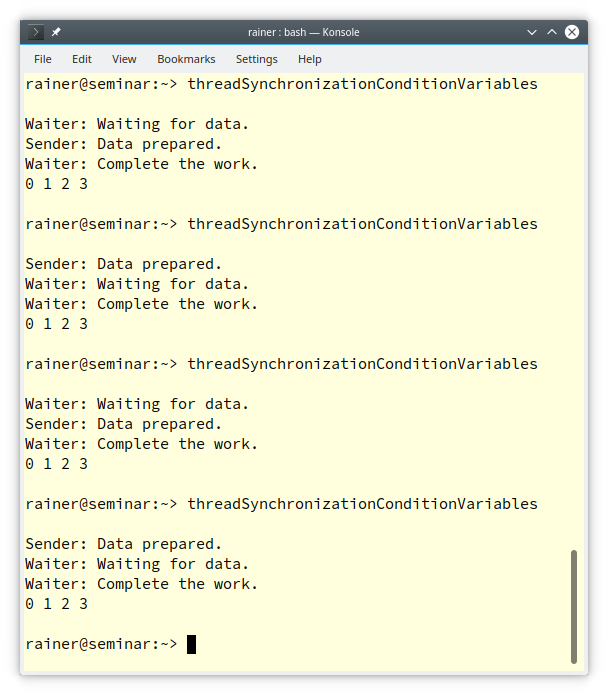
\includegraphics[width=0.8\textwidth]{content/3/chapter6/images/12.png}\\
\end{center}

条件变量有许多已知的问题。例如,接收者可能在没有通知的情况下唤醒,或者可能丢失通知。第一个问题称为伪唤醒,第二个问题称为未唤醒。谓词可以杜绝这两种问题。若发送方在接收方处于等待状态且未使用谓词之前发送通知,则通知可能丢失,所以接收者等待的事情永远不会发生。这是一个死锁。在研究程序的输出时会发现,若不使用谓词,那么每次运行一秒就会死锁。当然,可以使用没有谓词的条件变量。

若想知道发送-接收工作流程和条件变量陷阱的细节,请阅读我的帖子\href{https://www.modernescpp.com/index.php/c-core-guidelines-be-aware-of-the-traps-of-condition-variables}{“C++核心指南:小心条件变量的陷阱”}。

接下来,让我使用future/promise来实现相同的工作流。

\hspace*{\fill} \\ %插入空行
\noindent
\textbf{6.2.3.3.2\hspace{0.2cm}future和promise}

promise可以关联future的发送值、异常或通知。下面是使用promise和future的相应工作流。

\begin{lstlisting}[style=styleCXX]
// threadSynchronizationPromiseFuture.cpp

#include <iostream>
#include <future>
#include <thread>
#include <vector>

std::vector<int> myVec{};

void prepareWork(std::promise<void> prom) {
	
	myVec.insert(myVec.end(), {0, 1, 0, 3});
	std::cout << "Sender: Data prepared." << '\n';
	prom.set_value();

}

void completeWork(std::future<void> fut){

	std::cout << "Waiter: Waiting for data." << '\n';
	fut.wait();
	myVec[2] = 2;
	std::cout << "Waiter: Complete the work." << '\n';
	for (auto i: myVec) std::cout << i << " ";
	std::cout << '\n';

}

int main() {

	std::cout << '\n';
	
	std::promise<void> sendNotification;
	auto waitForNotification = sendNotification.get_future();
	
	std::thread t1(prepareWork, std::move(sendNotification));
	std::thread t2(completeWork, std::move(waitForNotification));
	t1.join();
	t2.join();
	
	std::cout << '\n';

}
\end{lstlisting}

研究这个工作流时,会发现同步简化为几个基本部分:prom.set\_value()(第14行)和fut.wait()(第21行)。我跳过了这次运行的截图,结果应该与前面条件变量的运行结果相同。

这里有更多关于promise和future的信息,通常称为\href{https://www.modernescpp.com/index.php/tag/tasks}{task}。

\hspace*{\fill} \\ %插入空行
\noindent
\textbf{6.2.3.3.3\hspace{0.2cm}std::atomic\_flag}

现在,我直接从C++11跳到C++20。

\begin{lstlisting}[style=styleCXX]
// threadSynchronizationAtomicFlag.cpp

#include <atomic>
#include <iostream>
#include <thread>
#include <vector>

std::vector<int> myVec{};

std::atomic_flag atomicFlag{};

void prepareWork() {

	myVec.insert(myVec.end(), {0, 1, 0, 3});
	std::cout << "Sender: Data prepared." << '\n';
	atomicFlag.test_and_set();
	atomicFlag.notify_one();

}

void completeWork() {

	std::cout << "Waiter: Waiting for data." << '\n';
	atomicFlag.wait(false);
	myVec[2] = 2;
	std::cout << "Waiter: Complete the work." << '\n';
	for (auto i: myVec) std::cout << i << " ";
	std::cout << '\n';

}

int main() {

	std::cout << '\n';
	
	std::thread t1(prepareWork);
	std::thread t2(completeWork);
	
	t1.join();
	t2.join();
	
	std::cout << '\n';

}
\end{lstlisting}

准备工作的线程(第16行)将atomicFlag设置为true并发送通知。完成工作的线程等待通知。只有当atomicFlag等于true时,才会解除阻塞。

下面是使用Microsoft编译器运行该程序,并运行几次的截图。

\begin{center}
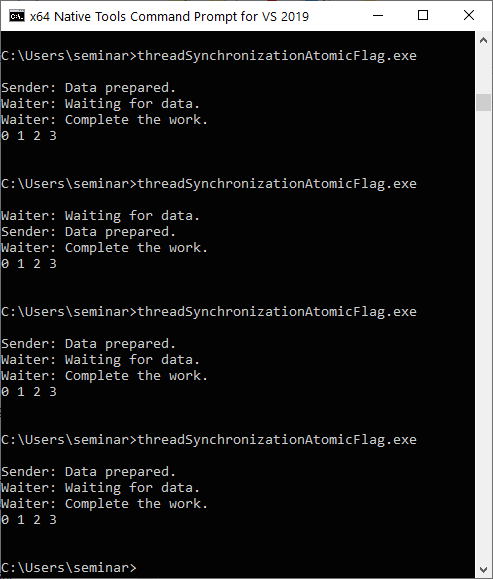
\includegraphics[width=0.8\textwidth]{content/3/chapter6/images/13.png}\\
\end{center}

\subsubsubsection{6.2.4\hspace{0.2cm}std::atomic扩展}

C++20中,std::atomic与\href{https://en.cppreference.com/w/cpp/atomic/atomic}{std::atomic\_ref}一样可以用浮点类型实例化,如float、double和long double。此外,std::atomic\_flag和std::atomic可以通过成员函数notify\_one、notify\_all和wait进行线程同步。通知和等待在std::atomic(布尔,整型,浮点和指针)和std::atomic\_ref的所有偏和全特化上都可用。

有了atomic<bool>,前面threadSynchronizationAtomicFlag.cpp可以重新进行实现。

\begin{lstlisting}[style=styleCXX]
// threadSynchronizationAtomicBool.cpp

#include <atomic>
#include <iostream>
#include <thread>
#include <vector>

std::vector<int> myVec{};

std::atomic<bool> atomicBool{false};

void prepareWork() {

	myVec.insert(myVec.end(), {0, 1, 0, 3});
	std::cout << "Sender: Data prepared." << '\n';
	atomicBool.store(true);
	atomicBool.notify_one();

}

void completeWork() {

	std::cout << "Waiter: Waiting for data." << '\n';
	atomicBool.wait(false);
	myVec[2] = 2;
	std::cout << "Waiter: Complete the work." << '\n';
	for (auto i: myVec) std::cout << i << " ";
	std::cout << '\n';

}

int main() {

	std::cout << '\n';
	
	std::thread t1(prepareWork);
	std::thread t2(completeWork);
	
	t1.join();
	t2.join();
	
	std::cout << '\n';

}
\end{lstlisting}

若atomicBool == false成立,则调用atomicBool.wait(false)将其阻塞,所以调用atomicBool.store(true)(第16行)将atomicBool设置为true并发送通知。

和前面一样,下面是使用Microsoft编译器编译,并运行四次运行。

\begin{center}
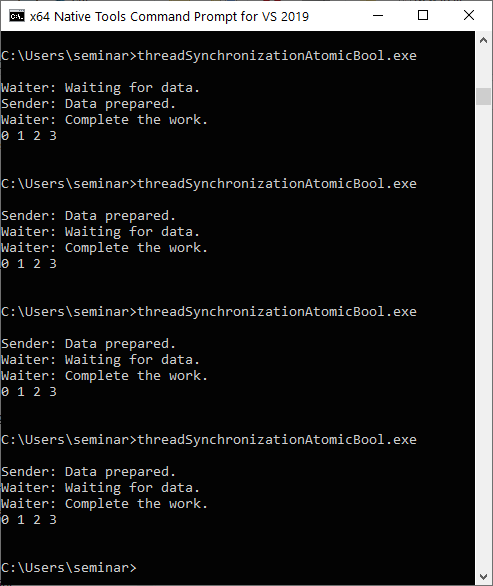
\includegraphics[width=0.8\textwidth]{content/3/chapter6/images/14.png}\\
\end{center}

\begin{tcolorbox}[breakable,enhanced jigsaw,colback=blue!5!white,colframe=blue!75!black,title={条件变量、promise/future对和std::atomic\_flag}]
	
当只需要一次性通知时(threadSynchronizationConditionVariable.cpp),promise/future对是比条件变量更好的选择,可以避免伪唤醒和未唤醒。此外,这种方式不需要使用锁或互斥量,也不需要使用谓词来防止伪唤醒或未唤醒。不过,其只有一个缺点:只能使用一次。

不确定我是否会使用promise/future对或原子类型(如std::atomic\_flag或std::atomic<bool>),来实现这样一个简单的线程同步工作流。从设计上讲,这些方式都是线程安全的,目前还不需要额外的保护机制。promise/future对更容易使用,不过原子类型可能运行的更快。但有一点是确定的,尽可能不要去使用条件变量。
	
\end{tcolorbox}


\begin{tcolorbox}[breakable,enhanced jigsaw,colback=mygreen!5!white,colframe=mygreen!75!black,title={总结}]
	
\begin{itemize}
\item 
std::atomic\_ref对引用的对象应用原子操作。并发写和读对于引用的对象来说是原子的,没有数据竞争。引用对象的生命周期必须超过std::atomic\_ref的生命周期。

\item 
std::shared\_ptr由一个控制块及其资源组成。控制块是线程安全的,但对资源的访问不是。C++20中,添加了原子共享指针:std::atomic<std::shared\_ptr<T>{}>和std::atomic<std::weak\_ptr<T>{}>。

\item 
std::atomic\_flag作为一种原子布尔值,是C++中唯一保证无锁的数据结构。其有限的接口在C++20中进行了扩展,现在可以返回它的值,并且可以将其用于线程同步。

\item 
std::atomic,在C++11中引入,并在C++20中得到了改进。可以为浮点值特化std::atomic,并且可以将其用于线程同步。
\end{itemize}
	
\end{tcolorbox}

\newpage








